\documentclass[11pt,table]{beamer}
\mode<presentation>
\usepackage{etex}
\usepackage{graphicx}
\usepackage{epstopdf}
\usepackage[english]{babel}
\usepackage{tabularx}
\usepackage{booktabs}
\usepackage{mathrsfs}
\usepackage{multicol}
\usepackage{bm}
\usepackage{subcaption}
\usepackage{wrapfig}
\usepackage{dcolumn}
\usepackage{threeparttable}
\usepackage{booktabs}
\usepackage{bbm}
\usepackage{amsmath,dsfont,listings}
\usepackage{amssymb}
\usepackage{rotating}
\usepackage{multirow}
\usepackage{tcolorbox}
\usepackage[authoryear]{natbib}
\usepackage{circledsteps}
\usepackage{qtree}

\usepackage{tikz}
\usetikzlibrary{arrows,decorations.pathmorphing,backgrounds,fit,positioning,shapes.symbols,chains}
\setbeamertemplate{section in toc}[sections numbered]
\setbeamertemplate{caption}[numbered]

\bibliographystyle{Econometrica}

\setbeamersize{text margin right=3.5mm, text margin left=7.5mm}  % text margin
\setbeamersize{sidebar width left=0cm, sidebar width right=0mm}
\setbeamertemplate{sidebar right}{}
\setbeamertemplate{sidebar left}{}

\definecolor{text-grey}{rgb}{0.45, 0.45, 0.45} % grey text on white background
\definecolor{bg-grey}{rgb}{0.66, 0.65, 0.60} % grey background (for white text)
\definecolor{fu-blue}{RGB}{0, 51, 102} % blue text
\definecolor{fu-green}{RGB}{153, 204, 0} % green text
\definecolor{fu-red}{RGB}{204, 0, 0} % red text (used by \alert)
\definecolor{BrewerBlue}{HTML}{377EB8} % Define Brewer Blue
\definecolor{BrewerRed}{HTML}{E41A1C}  % Define Brewer Red

\setbeamertemplate{frametitle}{%
    \vskip-30pt \color{text-grey}\large%
    \begin{minipage}[b][23pt]{\textwidth}%
    \flushleft\insertframetitle%
    \end{minipage}%
}

\setbeamertemplate{navigation symbols}{} 

%%% begin title page
\setbeamertemplate{title page}{
\vskip2pt\hfill
\vskip19pt\hskip3pt

% set the title and the author
\vskip4pt
\parbox[top][1.35cm][c]{11cm}{\LARGE\color{text-grey} \textcolor{red1}{RL}earning:\\[1ex] \inserttitle \\[1ex] \small \quad \\[3ex]}
\vskip17pt
\parbox[top][1.35cm][c]{11cm}{\small Unit 3-2: \insertsubtitle \\[2ex] \insertauthor \\[1ex]}
}
%%% end title page

%%% colors
\usecolortheme{lily}
\setbeamercolor*{normal text}{fg=black,bg=white}
\setbeamercolor*{alerted text}{fg=fu-red}
\setbeamercolor*{example text}{fg=fu-green}
\setbeamercolor*{structure}{fg=fu-blue}

\setbeamercolor*{block title}{fg=white,bg=black!50}
\setbeamercolor*{block title alerted}{fg=white,bg=black!50}
\setbeamercolor*{block title example}{fg=white,bg=black!50}

\setbeamercolor*{block body}{bg=black!10}
\setbeamercolor*{block body alerted}{bg=black!10}
\setbeamercolor*{block body example}{bg=black!10}

\setbeamercolor{bibliography entry author}{fg=fu-blue}
\setbeamercolor{bibliography entry journal}{fg=text-grey}
\setbeamercolor{item}{fg=fu-blue}
\setbeamercolor{navigation symbols}{fg=text-grey,bg=bg-grey}
%%% end colors

%%% headline
\setbeamertemplate{headline}{
\vskip30pt
}
%%% end headline

%%% footline
\newcommand{\footlinetext}{
%\insertshortinstitute, \insertshorttitle, \insertshortdate
}
\setbeamertemplate{footline}{
\vskip2pt
\hfill \raisebox{-1pt}{\usebeamertemplate***{navigation symbols}}
\hfill \insertframenumber\hspace{10pt}
\vskip4pt
}
%%% end footline

%%% settings for listings package
\lstset{extendedchars=true, showstringspaces=false, basicstyle=\footnotesize\sffamily, tabsize=2, breaklines=true, breakindent=10pt, frame=l, columns=fullflexible}
\lstset{language=Java} % this sets the syntax highlighting
\lstset{mathescape=true} % this switches on $...$ substitution in code
% enables UTF-8 in source code:
\lstset{literate={ä}{{\"a}}1 {ö}{{\"o}}1 {ü}{{\"u}}1 {Ä}{{\"A}}1 {Ö}{{\"O}}1 {Ü}{{\"U}}1 {ß}{\ss}1}
%%% end listings

\usepackage{concmath}
\usepackage{xcolor}
\definecolor{red1}{RGB}{206, 17, 38}
\definecolor{blue1}{RGB}{16, 118, 208}
\definecolor{gray1}{RGB}{117, 115, 115}
\usepackage{hyperref}


\newtheorem{proposition}{Proposition}
\newtheorem{assumption}{Definition}

\title[]{Short guides to reinforcement learning}
\subtitle[]{Monte Carlo Learning}
\author[D. Rostam-Afschar]{\textcolor{gray1}{Davud Rostam-Afschar (Uni Mannheim)}}
\date[]{\today}
\subject{Econometrics}
\renewcommand{\footlinetext}{\insertshortinstitute, \insertshorttitle, \insertshortdate}
\hypersetup{
    bookmarks=false,
    unicode=false,
    pdftoolbar=false,
    pdffitwindow=true,
    pdftitle={Reinforcement Learning for Business, Economics, and Social Sciences: \insertsubtitle},
    pdfauthor={Davud Rostam-Afschar},
    pdfsubject={Reinforcement Learning},
    pdfkeywords={reinforcement learning, Monte Carlo Learning},
    pdfnewwindow=true,
}
\def\sym#1{\ifmmode^{#1}\else\(^{#1}\)\fi}

\begin{document}

\begin{frame}[plain]
  \titlepage
\end{frame}

% --------------------------------------------------- Slide --
%\begin{frame}
	%\frametitle{Content}
	%\tableofcontents[]
%\end{frame}

\section{Monte Carlo Learning}
{
\setbeamercolor{background canvas}{bg=BrewerBlue}
\begin{frame}
\centering
\Huge
\textcolor{white}{How to learn from episodes?}
\thispagestyle{empty}
\end{frame}
}


\begin{frame}{RL Algorithms}
\only<1>{
Dynamic Programming Backup
\begin{figure}
	\centering
		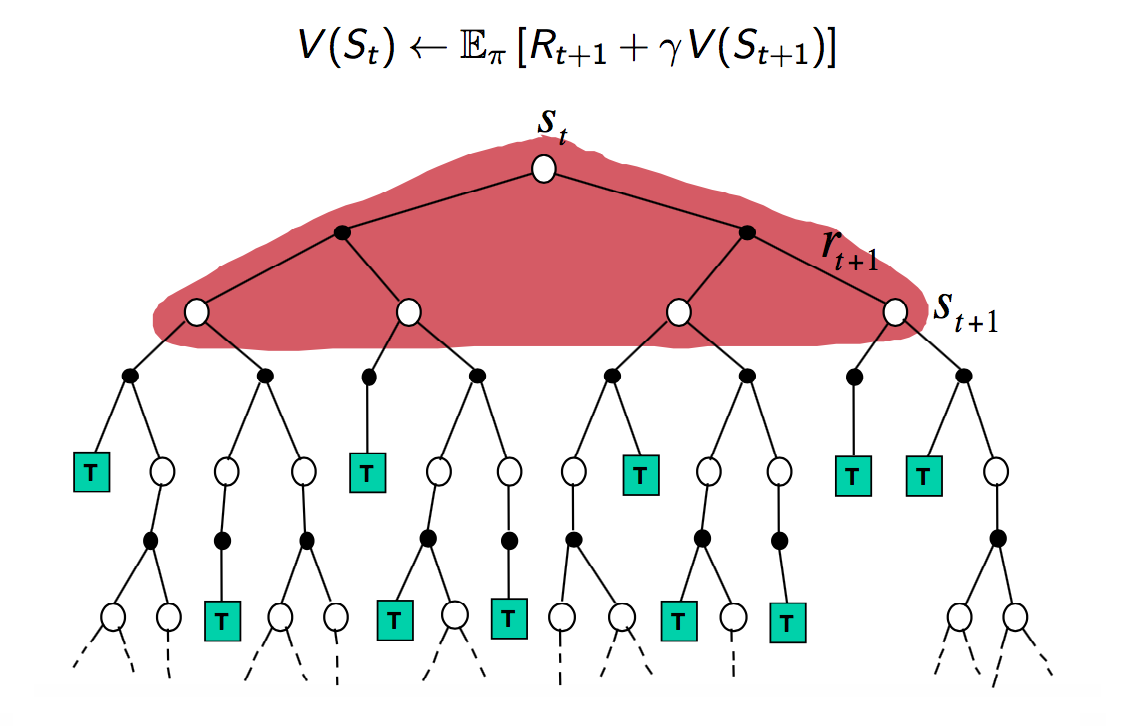
\includegraphics[width=0.60\textwidth]{figures/dynamic_programming_backup.png}
	\label{fig:DP}
\end{figure}
}
\only<2>{
Monte Carlo Backup
\begin{figure}
	\centering
		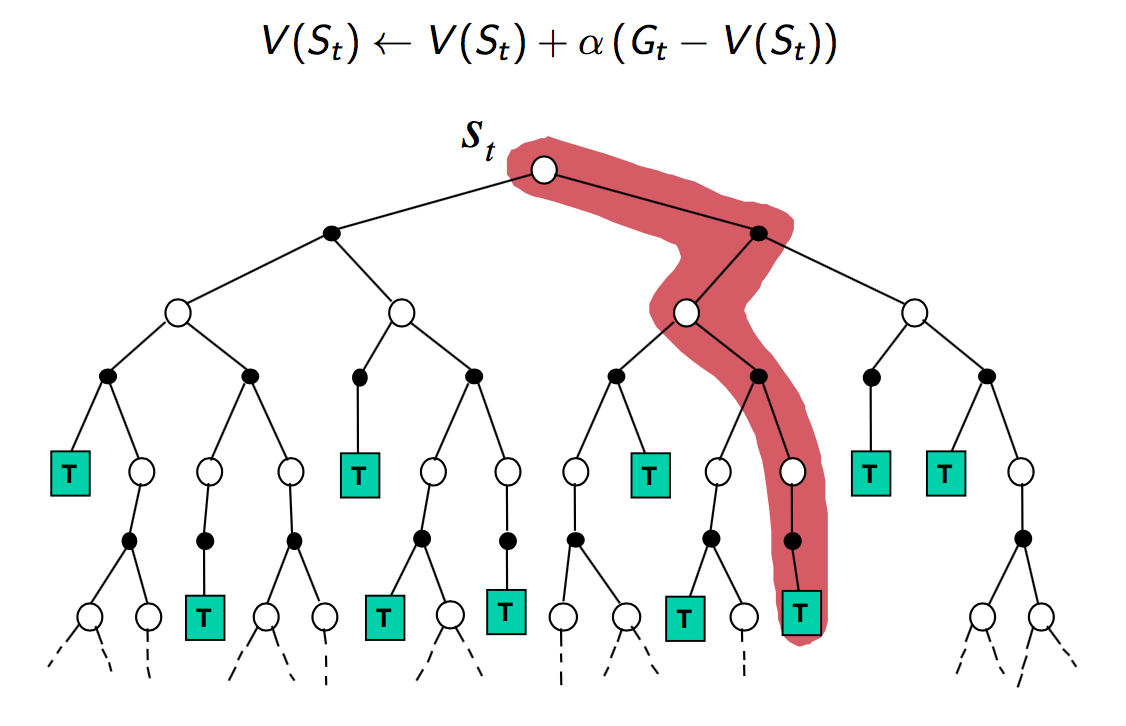
\includegraphics[width=0.60\textwidth]{figures/monte_carlo_backup.png}
	\label{fig:MC}
\end{figure}
}
\only<3>{
Temporal Difference Backup
\begin{figure}
	\centering
		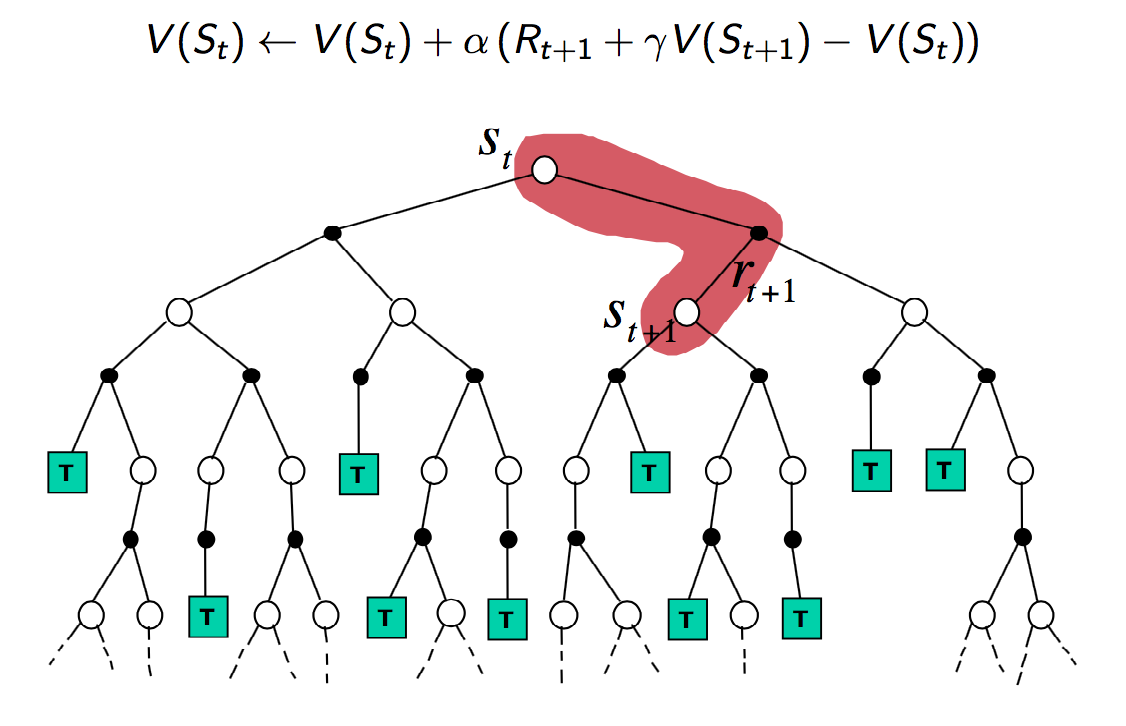
\includegraphics[width=0.60\textwidth]{figures/temporal_difference_backup.png}
	\label{fig:TD}
\end{figure}
}
\medskip
\hfill\footnotesize\textit{Source: David Silver}
\end{frame}


\begin{frame}{Model Free Evaluation}

\begin{itemize}
    \item Given a policy $\pi$ estimate $V^{\pi}(s)$ without any transition\\ or reward model

\item \textbf{Monte Carlo} evaluation
$$
\begin{aligned}
& V^{\pi}(s)=\mathbb{E}_{\pi}\left[\sum_{t} \gamma^{t} r_{t}\right] \\
& \textcolor{red1}{\approx \frac{1}{n(s)} \sum_{k=1}^{n(s)}\left[\sum_{t} \gamma^{t} r^{(k)}_{t}\right] \quad \text { (sample approximation) }}
\end{aligned}
$$

\end{itemize}
    
\end{frame}


\begin{frame}{Toy Maze Example}


\begin{columns}[T]
\begin{column}{0.45\textwidth}
\centering
\scalebox{0.6}{

\begin{tikzpicture}[line cap=round,line join=round,x=0.75pt,y=0.75pt,yscale=-1,xscale=1]

%Shape: Rectangle [id:dp08468554766918346] 
\draw  [fill=BrewerBlue] (240.34,110.03) -- (300.07,110.03) -- (300.07,169.77) -- (240.34,169.77) -- cycle ;
\draw[line width=2pt]   (180.53,50) -- (420.11,50) -- (420.11,229.53) -- (180.53,229.53) -- cycle ;
%Straight Lines [id:da4224686848111512] 
\draw[line width=1.5pt]    (240.03,49.53) -- (239.53,229.03) ;
%Straight Lines [id:da6046918343336376] 
\draw[line width=1.5pt]    (300.03,49.53) -- (299.53,229.53) ;
%Straight Lines [id:da9626667234054846] 
\draw[line width=1.5pt]   (360.03,50.03) -- (359.53,229.53) ;
%Straight Lines [id:da267347571646644] 
\draw[line width=1.5pt]    (180.11,110) -- (419.53,110.53) ;
%Straight Lines [id:da6745979138164762] 
\draw[line width=1.5pt]    (180.03,169.53) -- (420.11,170) ;
%Shape: Square [id:dp1839161508205971] 

% Text Node
\draw (159.47,68) node [anchor=north west][inner sep=0.75pt]   [align=left] {{\Large $3$}};
% Text Node
\draw (159.47,130) node [anchor=north west][inner sep=0.75pt]   [align=left] {{\Large $2$}};
% Text Node
\draw (159.47,186) node [anchor=north west][inner sep=0.75pt]   [align=left] {\textbf{{\Large $1$}}};
% Text Node
\draw (201.47,234) node [anchor=north west][inner sep=0.75pt]   [align=left] {{\Large $1$}};
% Text Node
\draw (263.47,234) node [anchor=north west][inner sep=0.75pt]   [align=left] {{\Large $2$}};
% Text Node
\draw (325.47,234) node [anchor=north west][inner sep=0.75pt]   [align=left] {{\Large $3$}};
% Text Node
\draw (381.47,234) node [anchor=north west][inner sep=0.75pt]   [align=left] {{\Large $4$}};
% Text Node
\draw (202.47,70) node [anchor=north west][inner sep=0.75pt]  [font=\huge] [align=left] {{\textbf{r}}};
% Text Node
\draw (264.47,70) node [anchor=north west][inner sep=0.75pt]  [font=\huge] [align=left] {{\huge \textbf{r}}};
% Text Node
\draw (324.47,70) node [anchor=north west][inner sep=0.75pt]  [font=\huge] [align=left] {{\huge \textbf{r}}};
% Text Node
\draw (370.47,70) node [anchor=north west][inner sep=0.75pt]  [font=\huge] [align=left] {$\boldsymbol{+1}$};
% Text Node
\draw (202.47,131) node [anchor=north west][inner sep=0.75pt]  [font=\huge] [align=left] {\textbf{u}};
% Text Node
\draw (322,131) node [anchor=north west][inner sep=0.75pt]  [font=\huge] [align=left] {\textbf{u}};
% Text Node
\draw (370.47,131) node [anchor=north west][inner sep=0.75pt]  [font=\huge] [align=left] {$\boldsymbol{-1}$};
% Text Node
\draw (202.47,188) node [anchor=north west][inner sep=0.75pt]  [font=\huge] [align=left] {\textbf{u}};
% Text Node
\draw (260,186) node [anchor=north west][inner sep=0.75pt]  [font=\huge] [align=left] {\textbf{l}};
% Text Node
\draw (322,186) node [anchor=north west][inner sep=0.75pt]  [font=\huge] [align=left] {\textbf{l}};
% Text Node
\draw (383,186) node [anchor=north west][inner sep=0.75pt]  [font=\huge] [align=left] {\textbf{l}};
\end{tikzpicture}
}
\end{column}
\begin{column}{0.55\textwidth}
Start state: (1,1)\\
Terminal states: (4,2), (4,3)  
\\No discount: $\gamma$=1

\vspace{2mm}
Reward is -0.04 for  non-terminal states

\end{column}
\end{columns}

\vspace{6mm}
\centering
\begin{columns}
\begin{column}{0.4\textwidth}

Four actions:
\begin{itemize}
	\item up (\textbf{u}),
	\item left (\textbf{l}),
	\item right (\textbf{r}),
	\item down (\textbf{d})
\end{itemize}
\end{column}
\begin{column}{0.6\textwidth}
Do not know the transition probabilities

\vspace{3mm}
  \textcolor{red1}{What is the value $V(s)$ of being in state $s$}
\end{column}
\end{columns}
    
\end{frame}

\section{Monte Carlo Evaluation}
{
\setbeamercolor{background canvas}{bg=BrewerBlue}
\begin{frame}
\centering
\Huge
\textcolor{white}{Monte Carlo Evaluation}
\thispagestyle{empty}
\end{frame}
}


\begin{frame}{Monte Carlo Evaluation}
\scriptsize
\begin{itemize}
    \item Let $G_{k}$ be a one-trajectory Monte Carlo target
$$
G_{k}=\sum_{t} \gamma^{t} r_{t}^{(k)}
$$
\uncover<2->{
\item First sample $(k=1)$ :
$$
\begin{aligned}
& \quad(1,1) \rightarrow(1,2) \rightarrow(1,3) \rightarrow(1,2) \rightarrow(1,3) \rightarrow(2,3) \rightarrow(3,3) \rightarrow(4,3) \\
& \quad-0.04-0.04-0.04-0.04-0.04-0.04-0.04+1 \\
& G_{1}=0.72
\end{aligned}
$$
}
\uncover<3->{
\item Second sample $(k=2)$ :
$$
\begin{aligned}
& \quad(1,1) \rightarrow(1,2) \rightarrow(1,3) \rightarrow(2,3) \rightarrow(3,3) \rightarrow(3,2) \rightarrow(3,3) \rightarrow(4,3) \\
& \quad-0.04-0.04-0.04-0.04-0.04-0.04-0.04+1 \\
& G_{2}=0.72
\end{aligned}
$$ 
}
\end{itemize}

\begin{columns}[T]
\begin{column}{0.6\textwidth}
\uncover<4>{
\begin{itemize}
   \item Third sample $(k=3)$:
$$
\begin{aligned}
& (1,1) \rightarrow(2,1) \rightarrow(3,1) \rightarrow(3,2) \rightarrow(4,2) \\
& -0.04-0.04-0.04-0.04-1 \\
& G_{3}=-1.16
\end{aligned}
$$
\end{itemize}
}
\end{column}
\begin{column}{0.4\textwidth}
\centering
\vspace{-8mm}
\scalebox{0.6}{

\begin{tikzpicture}[line cap=round,line join=round,x=0.75pt,y=0.75pt,yscale=-1,xscale=1]

%Shape: Rectangle [id:dp08468554766918346] 
\draw  [fill=BrewerBlue] (240.34,110.03) -- (300.07,110.03) -- (300.07,169.77) -- (240.34,169.77) -- cycle ;
\draw[line width=2pt]   (180.53,50) -- (420.11,50) -- (420.11,229.53) -- (180.53,229.53) -- cycle ;
%Straight Lines [id:da4224686848111512] 
\draw[line width=1.5pt]    (240.03,49.53) -- (239.53,229.03) ;
%Straight Lines [id:da6046918343336376] 
\draw[line width=1.5pt]    (300.03,49.53) -- (299.53,229.53) ;
%Straight Lines [id:da9626667234054846] 
\draw[line width=1.5pt]   (360.03,50.03) -- (359.53,229.53) ;
%Straight Lines [id:da267347571646644] 
\draw[line width=1.5pt]    (180.11,110) -- (419.53,110.53) ;
%Straight Lines [id:da6745979138164762] 
\draw[line width=1.5pt]    (180.03,169.53) -- (420.11,170) ;
%Shape: Square [id:dp1839161508205971] 

% Text Node
\draw (159.47,68) node [anchor=north west][inner sep=0.75pt]   [align=left] {{\Large $3$}};
% Text Node
\draw (159.47,130) node [anchor=north west][inner sep=0.75pt]   [align=left] {{\Large $2$}};
% Text Node
\draw (159.47,186) node [anchor=north west][inner sep=0.75pt]   [align=left] {\textbf{{\Large $1$}}};
% Text Node
\draw (201.47,234) node [anchor=north west][inner sep=0.75pt]   [align=left] {{\Large $1$}};
% Text Node
\draw (263.47,234) node [anchor=north west][inner sep=0.75pt]   [align=left] {{\Large $2$}};
% Text Node
\draw (325.47,234) node [anchor=north west][inner sep=0.75pt]   [align=left] {{\Large $3$}};
% Text Node
\draw (381.47,234) node [anchor=north west][inner sep=0.75pt]   [align=left] {{\Large $4$}};
% Text Node
\draw (202.47,70) node [anchor=north west][inner sep=0.75pt]  [font=\huge] [align=left] {{\textbf{r}}};
% Text Node
\draw (264.47,70) node [anchor=north west][inner sep=0.75pt]  [font=\huge] [align=left] {{\huge \textbf{r}}};
% Text Node
\draw (324.47,70) node [anchor=north west][inner sep=0.75pt]  [font=\huge] [align=left] {{\huge \textbf{r}}};
% Text Node
\draw (370.47,70) node [anchor=north west][inner sep=0.75pt]  [font=\huge] [align=left] {$\boldsymbol{+1}$};
% Text Node
\draw (202.47,131) node [anchor=north west][inner sep=0.75pt]  [font=\huge] [align=left] {\textbf{u}};
% Text Node
\draw (322,131) node [anchor=north west][inner sep=0.75pt]  [font=\huge] [align=left] {\textbf{u}};
% Text Node
\draw (370.47,131) node [anchor=north west][inner sep=0.75pt]  [font=\huge] [align=left] {$\boldsymbol{-1}$};
% Text Node
\draw (202.47,188) node [anchor=north west][inner sep=0.75pt]  [font=\huge] [align=left] {\textbf{u}};
% Text Node
\draw (260,186) node [anchor=north west][inner sep=0.75pt]  [font=\huge] [align=left] {\textbf{l}};
% Text Node
\draw (322,186) node [anchor=north west][inner sep=0.75pt]  [font=\huge] [align=left] {\textbf{l}};
% Text Node
\draw (383,186) node [anchor=north west][inner sep=0.75pt]  [font=\huge] [align=left] {\textbf{l}};
\end{tikzpicture}
}
\end{column}
\end{columns}
    
\end{frame}



\begin{frame}{Monte Carlo Evaluation}
%\scriptsize
\begin{itemize}
    \item Let $G_{k}$ be a \emph{one-trajectory} Monte Carlo target $G_{k}=\sum_{t} \gamma^{t} r_{t}^{(k)}$

\item Approximate value function

$$
\begin{gathered}
V_{n}^{\pi}(s) \approx \frac{1}{n(s)} \sum_{k=1}^{n(s)} G_{k} \\\pause
=\frac{1}{n(s)}\left(G_{n(s)}+\sum_{k=1}^{n(s)-1} G_{k}\right) \\
=\frac{1}{n(s)}\left(G_{n(s)}+(n(s)-1) V_{n-1}^{\pi}(s)\right) \\
=V_{n-1}^{\pi}(s)+\frac{1}{n(s)}\left(G_{n(s)}-V_{n-1}^{\pi}(s)\right)
\end{gathered}
\pause
$$
\item \textbf{Incremental update}
$$
\textcolor{red1}{V_{n}^{\pi}(s) \leftarrow V_{n-1}^{\pi}(s)+\alpha_{n}\left(G_{n}-V_{n-1}^{\pi}(s)\right),}
$$ 
where $\alpha_{n}=$ learning rate 1/$n(s)$
\end{itemize}
    
\end{frame}


\begin{frame}{Exploration vs Exploitation}
Stochastic approximation (Robbins-Monro algorithm)
\begin{itemize}

\item \textbf{Theorem}: If $\alpha_{n}$ is appropriately decreased with number of times a state is visited then $V_{n}^{\pi}(s)$ converges to correct value

\item \textbf{Sufficient conditions} for $\alpha_{n}$ :


\begin{align}
&  \sum_{n} \alpha_{n} \rightarrow \infty \\
& \sum_{n} \alpha^2_{n} < \infty
\end{align}

\item \text Often $\alpha_{n}(s)=1 / n(s)$, where $n(s)=$ \# of times $s$ is visited 
   \end{itemize} 
	\pause
	\footnotesize
	\begin{table}[ht]
    \centering
    \begin{tabular}{rr}
    \hline
    $n(s)$ & $\alpha_{n}$ \\ 
    \hline
    2  & 50\%   \\ \pause
    5  & 20\%   \\ \pause
    10 & 10\%   \\ \pause
    20 & 5\%    \\ \pause
    40 & 2.5\%  \\ \pause
    80 & 1.25\% \\ 
    \hline
    \end{tabular}
\end{table}
\end{frame}



\begin{frame}{First-visit Monte Carlo (MC) Evaluation}


\begin{tcolorbox}[colframe=black, boxrule=1pt, sharp corners]

\textcolor{red1}{MCevaluation $\left(\pi, V^{\pi}\right)$}

\quad Initialize 

\qquad 
\(\pi \leftarrow\) policy to be evaluated

\qquad 
\(V^{\pi}(s) \leftarrow\) arbitrary state‐value function

\qquad 
\(n(s)\leftarrow 0,\;\forall\,s\in\mathcal{S}\)

\quad Repeat

\qquad Generate the $k$th episode using $\pi(s)$

\qquad For each state \(t\) appearing in the episode 

\qquad Return $r$ following the first occurrence of \(t\)

\qquad Update counts: $n(s) \leftarrow n(s)+1$

\qquad Learning rate: $\alpha \leftarrow 1 / n(s)$

\qquad Update value: $V^{\pi}(s) \leftarrow V^{\pi}(s)+\alpha\left(\sum_{t} \gamma^{t} r_{t}^{(k)}-V^{\pi}(s)\right)$

\quad Until convergence of $V^{\pi}$

\quad Return $V^{\pi}$


\end{tcolorbox}
    
\end{frame}

\section{Monte Carlo Control}
{
\setbeamercolor{background canvas}{bg=BrewerBlue}
\begin{frame}
\centering
\Huge
\textcolor{white}{Monte Carlo Control}
\thispagestyle{empty}
\end{frame}
}


\begin{frame}{Monte Carlo Control}


\begin{itemize}
    \item Let $G_{k}^{a}$ be a one-trajectory Monte Carlo target


$$
G_{k}^{a}=\underbrace{r_{0}^{(k)}}_{a}+\underbrace{\sum_{t=1} \gamma_{\pi}^{t} r_{t}^{(k)}}_{\pi}
$$

\item Alternate between

\begin{itemize}
     
\item  \textbf{Policy evaluation}

$$
\textcolor{red1}{Q_{n}^{*}(s, a) \leftarrow Q_{n-1}^{\pi}(s, a)+\alpha_{n}\left(G_{k}^{a}-Q_{n-1}^{\pi}(s, a)\right)}
$$
\item  \textbf{Policy improvement}

$$
\textcolor{red1}{\pi^{\prime}(s) \leftarrow \underset{a}{\operatorname{argmax}} Q^{\pi}(s, a)}
$$ 
\end{itemize}
    \end{itemize}
\end{frame}


%
%\begin{frame}{Comparison}
%
%
    %\begin{itemize}
        %\item \textbf{Monte Carlo evaluation}:
%\begin{itemize}
%\item \textcolor{teal}{Unbiased estimate}
%\item \textcolor{red1}{High variance}
%\item \textcolor{red1}{Needs many trajectories}\\[2ex]
 %
%\end{itemize} 
%\item \textbf{Temporal difference evaluation}:
%\begin{itemize}
%\item \textcolor{red1}{Biased estimate}
%\item \textcolor{teal}{Lower variance}
%\item \textcolor{teal}{Needs less trajectories}
 %
%\end{itemize}
    %\end{itemize}
%\end{frame}


\begin{frame}[t,allowframebreaks
]\nocite{*}
\frametitle{References}
\footnotesize
\bibliography{bib}
\end{frame}
\section{Takeaways}
{
\setbeamercolor{background canvas}{bg=BrewerBlue}
\begin{frame}
\centering
\Huge
\textcolor{white}{Takeaways}
\thispagestyle{empty}
\end{frame}
}



\begin{frame}{How to Learn Values Using Monte Carlo Methods?}
  \begin{itemize}
    \item No need to know transition probabilities or reward function\\$\rightarrow$ Model free\\[2ex]
    \item Average returns from complete episodes under the target policy\\$\rightarrow$ Unbiased value estimation from samples\\[2ex]
    \item Revises estimates only after each episode using the observed return\\$\rightarrow$ Needs many trajectories
  \end{itemize}
\end{frame}

\end{document}
